\documentclass[aspectratio=169,10pt]{beamer}

\usepackage{iftex}
\ifPDFTeX
  \usepackage[T1]{fontenc}
  \usepackage[utf8]{inputenc}
\fi

\usetheme{Madrid}

\usepackage{amsmath,amssymb}
\usepackage{booktabs}
\usepackage{array}
\usepackage{graphicx}

\definecolor{brandblue}{RGB}{51,51,178}
\colorlet{mainblue}{brandblue}
\colorlet{darkblue}{brandblue!62!black}

\definecolor{cMain}{HTML}{1F2937}
\definecolor{cBlue}{HTML}{185FA5}
\definecolor{cRed}{HTML}{A32D2D}
\definecolor{cGreen}{HTML}{27500A}
\definecolor{cOrange}{HTML}{854F0B}
\definecolor{cGrey}{HTML}{5F5E5A}

\setbeamercolor{normal text}{fg=cMain}
\setbeamercolor{structure}{fg=mainblue}
\setbeamercolor{frametitle}{bg=mainblue,fg=white}
\setbeamercolor{palette primary}{bg=mainblue,fg=white}
\setbeamercolor{palette secondary}{bg=darkblue,fg=white}
\setbeamercolor{palette tertiary}{bg=darkblue,fg=white}
\setbeamercolor{palette quaternary}{bg=darkblue,fg=white}
\setbeamercolor{title}{fg=white,bg=mainblue}
\setbeamercolor{subtitle}{fg=white}
\setbeamercolor{alerted text}{fg=cRed}

\setbeamertemplate{navigation symbols}{}
\setbeamertemplate{blocks}[rounded][shadow=false]
\setbeamertemplate{itemize item}{\raisebox{0.15ex}{\scriptsize$\bullet$}}
\setbeamertemplate{itemize subitem}{\raisebox{0.15ex}{\tiny$\circ$}}

\setbeamerfont{title}{size=\LARGE}
\setbeamerfont{subtitle}{size=\large}
\setbeamerfont{block body}{size=\footnotesize}
\setbeamerfont{block title}{size=\small}
\setbeamerfont{itemize/enumerate body}{size=\footnotesize}
\setbeamerfont{itemize/enumerate subbody}{size=\scriptsize}
\setlength{\leftmargini}{1.15em}

\graphicspath{{../report/figures/}{../figures/}{./}}

\newcommand{\epsr}{\varepsilon_r}
\newcommand{\epseff}{\varepsilon_{\mathrm{eff}}}
\newcommand{\Cair}{C_{\mathrm{air}}}
\newcommand{\Zzero}{Z_0}
\newcolumntype{L}[1]{>{\raggedright\arraybackslash}p{#1}}
\newcommand{\MMSLTwoFit}{1.9956}
\newcommand{\MMSEnergyFit}{0.9983}
\newcommand{\RefSlopeROne}{0.6383}
\newcommand{\RefSlopeRTwo}{0.6230}
\newcommand{\HJDiscrepancyFEM}{0.88}
\newcommand{\HJDiscrepancyIPC}{1.61}


\title[Microstrip FEM]{2D Finite Element Analysis of a Microstrip Transmission Line}
\subtitle{A verified numerical evidence chain for capacitance and impedance}
\author[Project 2]{\texorpdfstring{Group C\\[0.4em]
  {\small Chuqiao Tang (2360692), Jinyu Ma (2363433)}\\
  {\small Muqing Xu (2362900), Shuoran Fu (2362626)}\\
  {\small Taiqi Zhang (2363684), Yujia Ding (2362094)}}{Group C: Chuqiao Tang, Jinyu Ma, Muqing Xu, Shuoran Fu, Taiqi Zhang, Yujia Ding}}
\institute[MTH321 Project 2]{MTH321 Numerical PDEs --- Project 2}
\date[October 2026]{October 2026}

\begin{document}

\maketitle

% ---------------------------------------------------------------------
\section{Problem}
% ---------------------------------------------------------------------

\begin{frame}{Problem and engineering goal}
  \begin{columns}[T]
    \begin{column}{0.50\textwidth}
      \begin{block}{What we need}
        \begin{itemize}
          \item Compute the quasistatic capacitance per unit length.
          \item Reuse the same mesh for the all-air capacitance.
          \item Convert the matched pair into $\epseff$ and $\Zzero$.
        \end{itemize}
      \end{block}
    \end{column}
    \begin{column}{0.46\textwidth}
      \begin{block}{What would not be enough}
        \begin{itemize}
          \item A single FEM number near $50\,\Omega$.
          \item Agreement with an empirical formula only.
          \item Unchecked corner and boundary effects.
        \end{itemize}
      \end{block}
    \end{column}
  \end{columns}
  \vspace{0.7em}
  \begin{alertblock}{Takeaway}
    The result matters because the numerical evidence chain makes it defensible.
  \end{alertblock}
\end{frame}

\begin{frame}{Geometry and PDE model}
  \begin{columns}[T]
    \begin{column}{0.48\textwidth}
      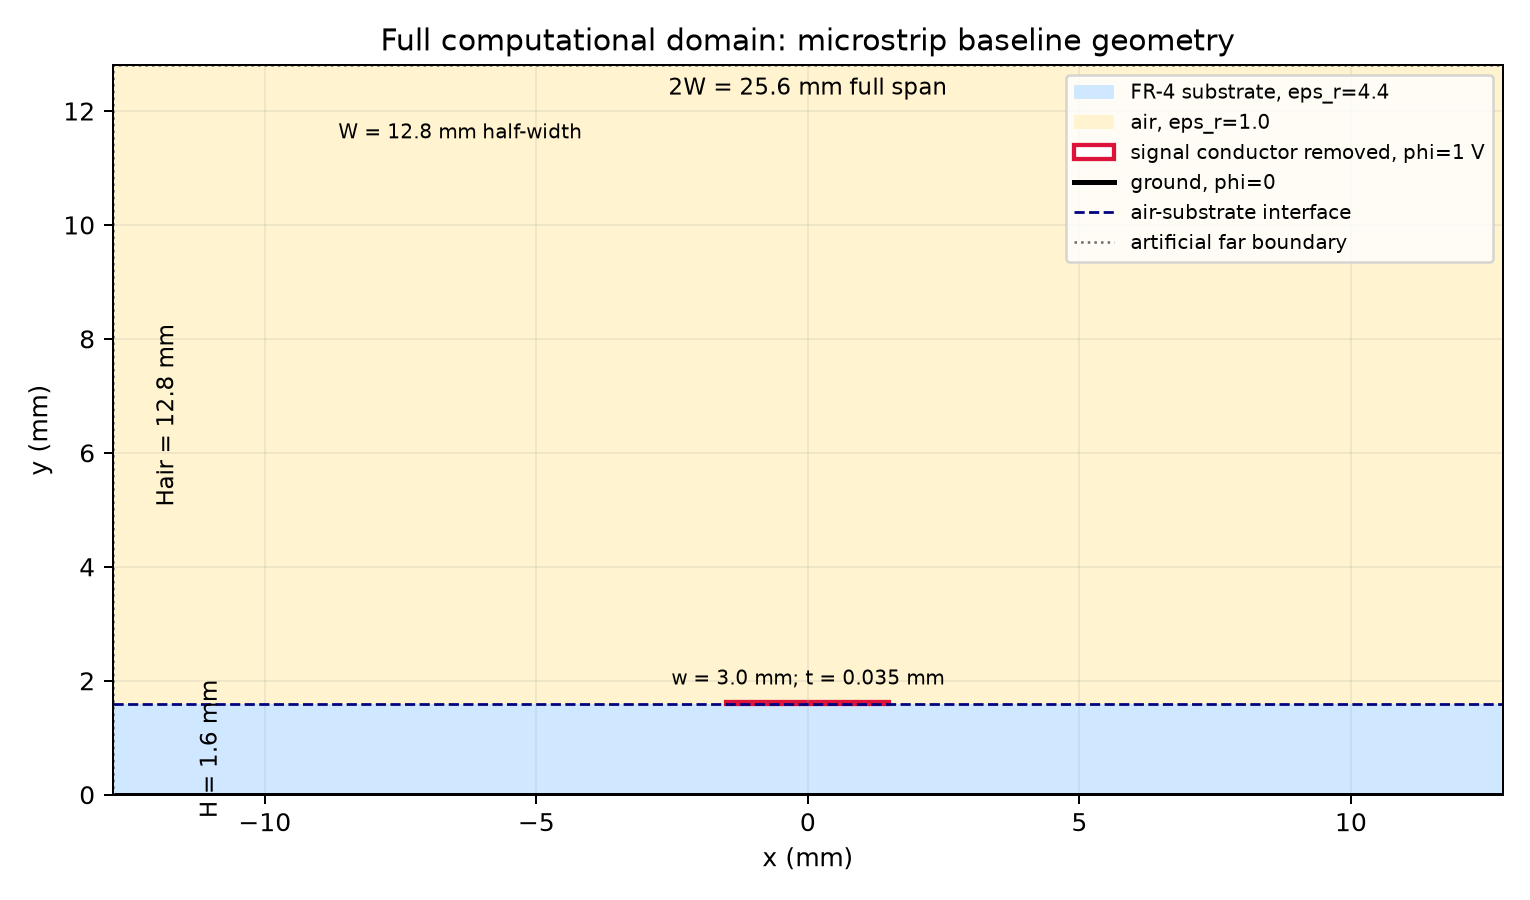
\includegraphics[width=\linewidth]{geometry_full_domain.png}
    \end{column}
    \begin{column}{0.48\textwidth}
      \begin{block}{Electrostatic model}
        \[
          -\nabla\cdot(\varepsilon\nabla\phi)=0
        \]
        \[
          \phi=1\,\mathrm{V}\ \text{on trace},\qquad
          \phi=0\ \text{on ground}
        \]
        Homogeneous Neumann conditions are used on the top and side artificial boundaries.
      \end{block}
      \begin{block}{Physical dimensions}
        $H=1.6\,\mathrm{mm}$, $w=3.0\,\mathrm{mm}$,
        $t=0.035\,\mathrm{mm}$, substrate $\epsr=4.4$.
      \end{block}
    \end{column}
  \end{columns}
\end{frame}

\begin{frame}{Weak form and P1 FEM}
  \begin{block}{Weak problem}
    Find $\phi\in V_g$ such that
    \[
      \int_{\Omega}\varepsilon\nabla\phi\cdot\nabla v\,d\Omega=0
      \quad\forall v\in V_0 .
    \]
  \end{block}
  \begin{columns}[T]
    \begin{column}{0.49\textwidth}
      \begin{block}{Discretisation}
        \begin{itemize}
          \item Conforming triangular $P_1$ elements.
          \item Trace interior removed from the field domain.
          \item Dirichlet dofs eliminated before solving.
        \end{itemize}
      \end{block}
    \end{column}
    \begin{column}{0.47\textwidth}
      \begin{block}{Material interface}
        $\phi_h$ is continuous across the air-substrate line. Flux balance is enforced weakly by elementwise integration of discontinuous $\varepsilon$.
      \end{block}
    \end{column}
  \end{columns}
  \vspace{0.35em}
  \begin{alertblock}{Takeaway}
    The model keeps the conductor boundary, material jump and artificial boundary conditions explicit.
  \end{alertblock}
\end{frame}

% ---------------------------------------------------------------------
\section{Verification}
% ---------------------------------------------------------------------

\begin{frame}{Solver verification: manufactured solution}
  \begin{columns}[T]
    \begin{column}{0.57\textwidth}
      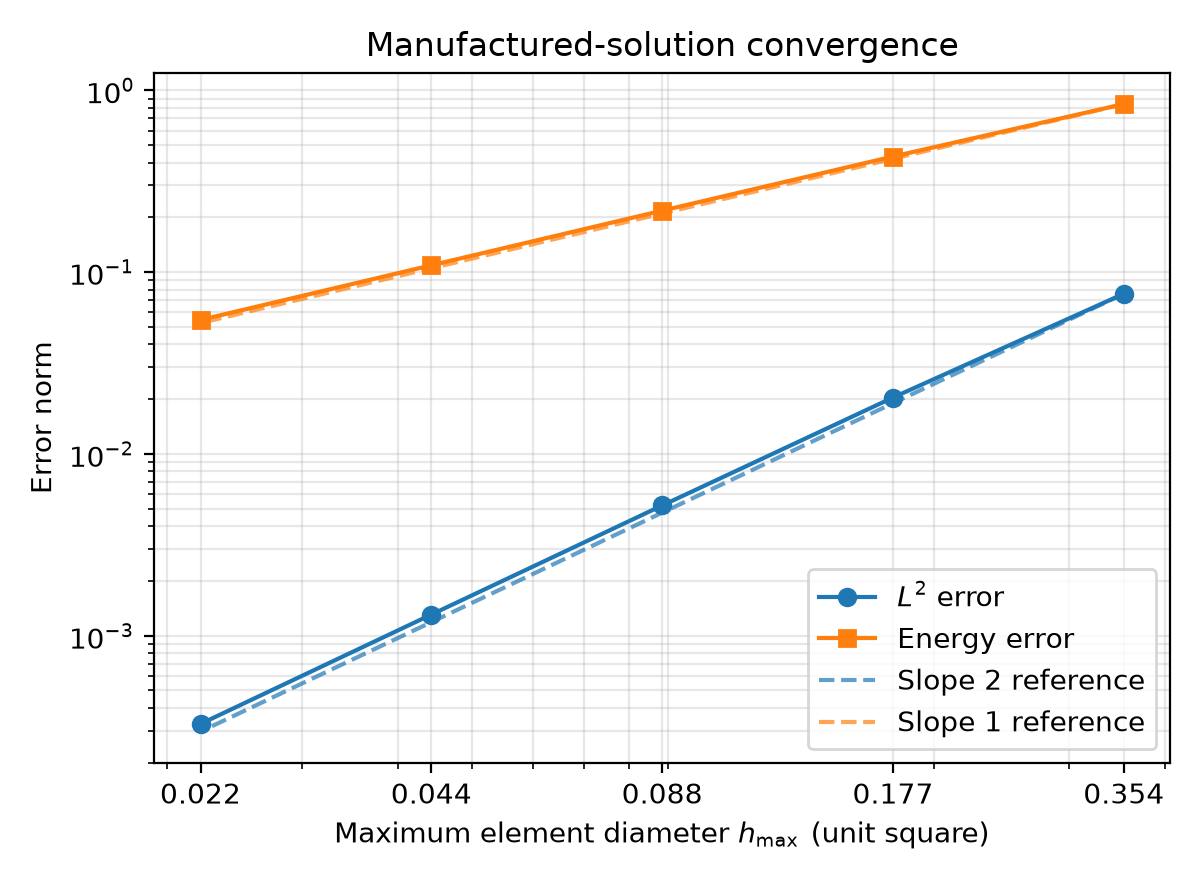
\includegraphics[width=0.93\linewidth]{mms_convergence_report.png}
    \end{column}
    \begin{column}{0.39\textwidth}
      \begin{block}{Known exact solution}
        \[
          u(x,y)=\sin(\pi x)\sin(\pi y)
        \]
        Observed rates: $p_{L^2}\approx2$, $p_E\approx1$.
      \end{block}
      \begin{block}{Microstrip baseline checks}
        \begin{tabular}{@{}lr@{}}
          Potential & $0\le\phi_h\le1$\\
          Symmetry error & $3.24\times10^{-14}$\\
          $\|r_F\|_\infty$ & $3.10\times10^{-25}$\\
          $\delta_{EQ}$ & $2.54\times10^{-15}$
        \end{tabular}
      \end{block}
    \end{column}
  \end{columns}
  \begin{alertblock}{Takeaway}
    MMS checks solver accuracy; baseline diagnostics check the assembled microstrip problem.
  \end{alertblock}
\end{frame}

\begin{frame}{Domain truncation and the 8H choice}
  \begin{columns}[T]
    \begin{column}{0.57\textwidth}
      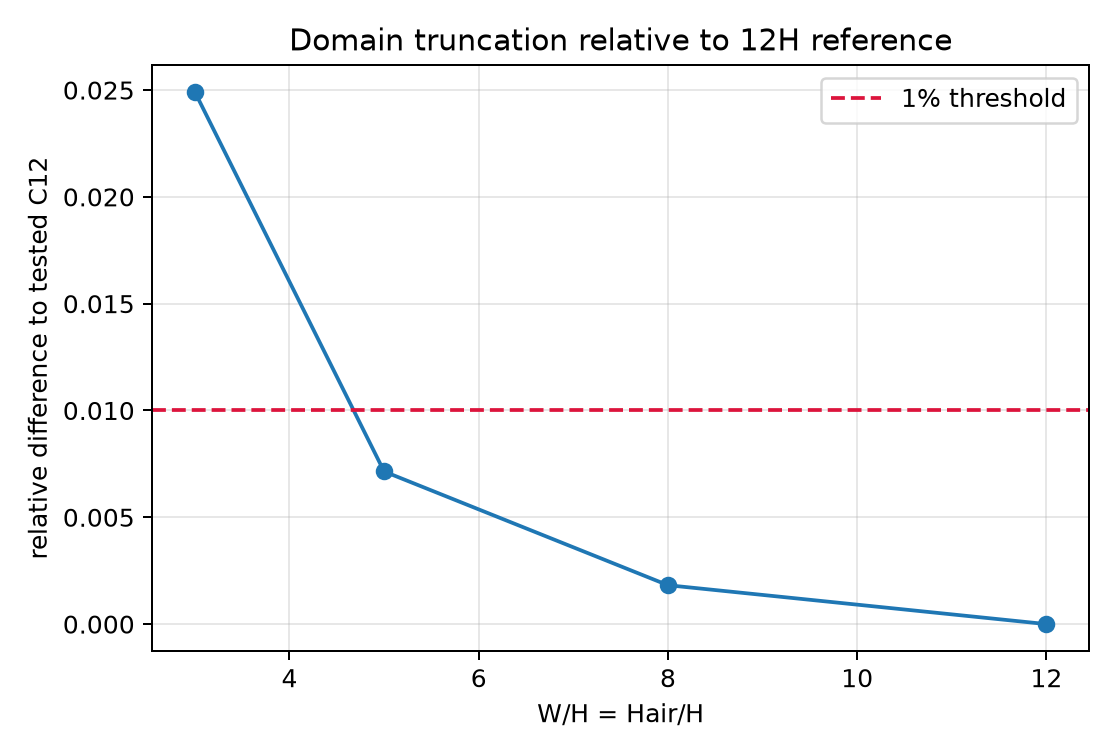
\includegraphics[width=\linewidth]{domain_truncation.png}
    \end{column}
    \begin{column}{0.39\textwidth}
      \begin{block}{Relative to tested 12H reference}
        \begin{tabular}{@{}lr@{}}
          \toprule
          Domain & Difference\\
          \midrule
          3H & $2.491\%$\\
          5H & $0.714\%$\\
          8H & $0.182\%$\\
          12H & reference\\
          \bottomrule
        \end{tabular}
      \end{block}
      \begin{block}{Mesh-adequacy repeat}
        Finer 12H repeat changed $C$ by about $0.0360\%$.
      \end{block}
    \end{column}
  \end{columns}
  \begin{alertblock}{Takeaway}
    The final 8H domain is a controlled cost-accuracy choice, not an assumed infinite-domain result.
  \end{alertblock}
\end{frame}

\begin{frame}{Corner singularity and uniform convergence}
  \begin{columns}[T]
    \begin{column}{0.58\textwidth}
      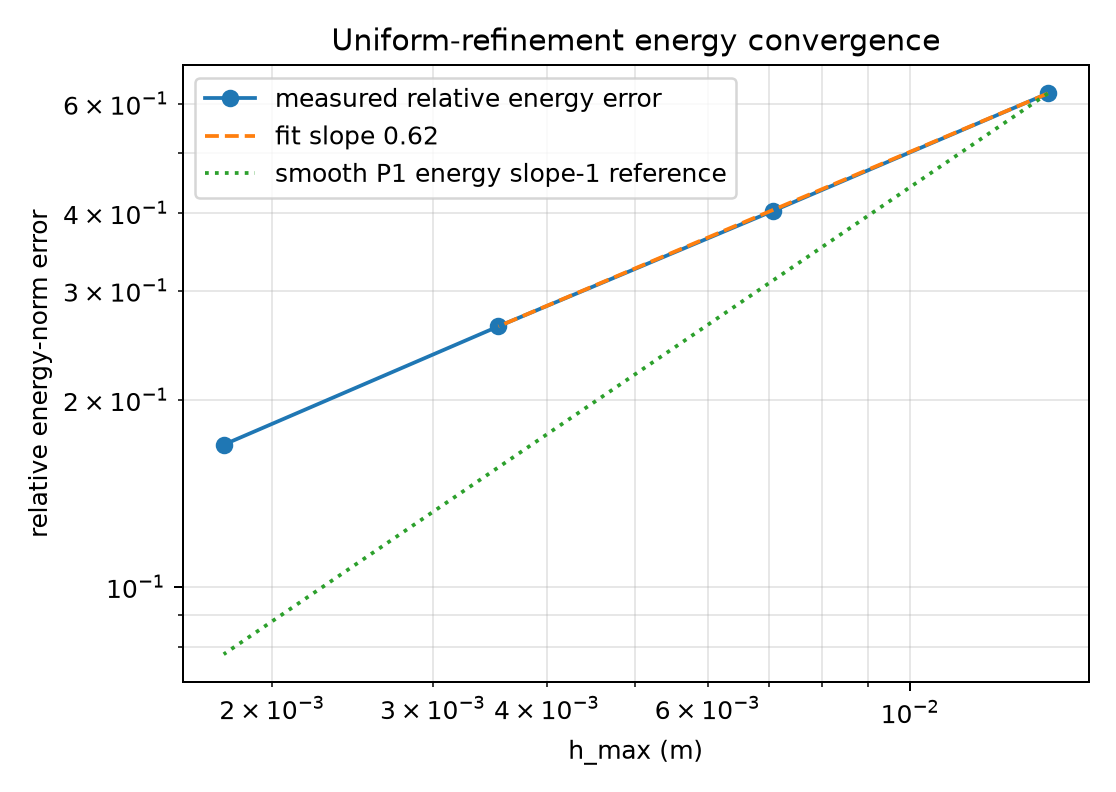
\includegraphics[width=0.94\linewidth]{uniform_energy_convergence.png}
    \end{column}
    \begin{column}{0.38\textwidth}
      \begin{block}{What limits the rate}
        \begin{itemize}
          \item Trace corners concentrate electric field.
          \item Lower corners also meet the material interface.
        \end{itemize}
      \end{block}
      \begin{block}{Observed energy fit}
        \[
          p_E \approx 0.623
        \]
      \end{block}
    \end{column}
  \end{columns}
  \begin{alertblock}{Takeaway}
    The reduced rate is consistent with corner- and interface-limited regularity.
  \end{alertblock}
\end{frame}

\begin{frame}{Uniform vs graded refinement}
  \begin{columns}[T]
    \begin{column}{0.63\textwidth}
      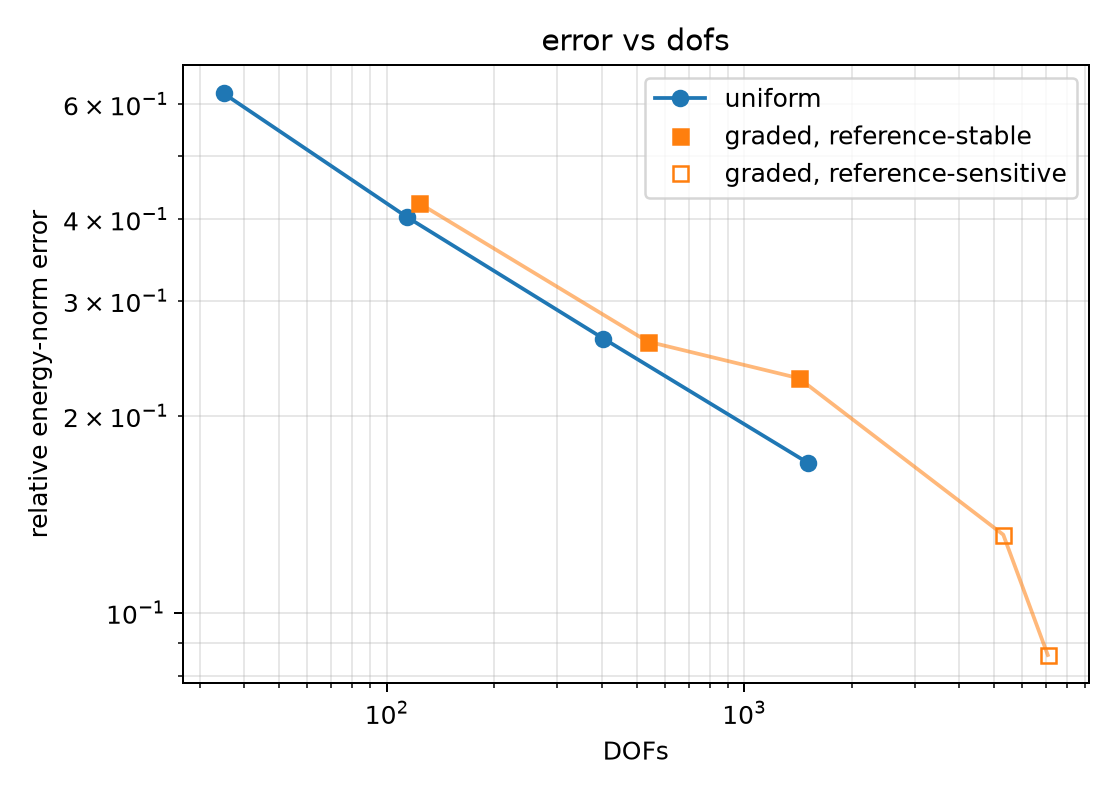
\includegraphics[width=\linewidth]{error_vs_dofs.png}
    \end{column}
    \begin{column}{0.33\textwidth}
      \begin{block}{Cost metrics checked}
        \begin{itemize}
          \item DOFs
          \item NNZ
          \item Measured median time
        \end{itemize}
      \end{block}
      \begin{block}{Reference-stable targets}
        Recorded relative errors: $0.40$ and $0.30$.
      \end{block}
      \begin{alertblock}{Result}
        Recorded estimates favoured uniform refinement in DOFs, NNZ and time. A new geometry audit requires common-overlay validation before precise efficiency claims.
      \end{alertblock}
    \end{column}
  \end{columns}
\end{frame}

\begin{frame}{Residual-driven adaptive refinement}
  \begin{columns}[T]
    \begin{column}{0.43\textwidth}
      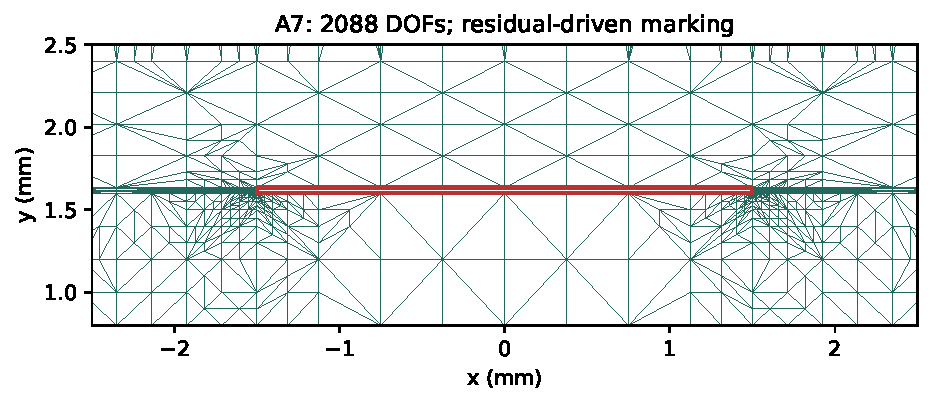
\includegraphics[width=\linewidth]{../figures/adaptive_extension/adaptive_final_mesh_slide.pdf}
      \begin{block}{Solution-driven marking}
        Flux-jump indicator; D\"orfler $\theta=0.5$.\\
        Primary: 404 to 2088 DOFs.\\
        Same $8H$ model, $P_1$ and direct solver.
      \end{block}
    \end{column}
    \begin{column}{0.55\textwidth}
      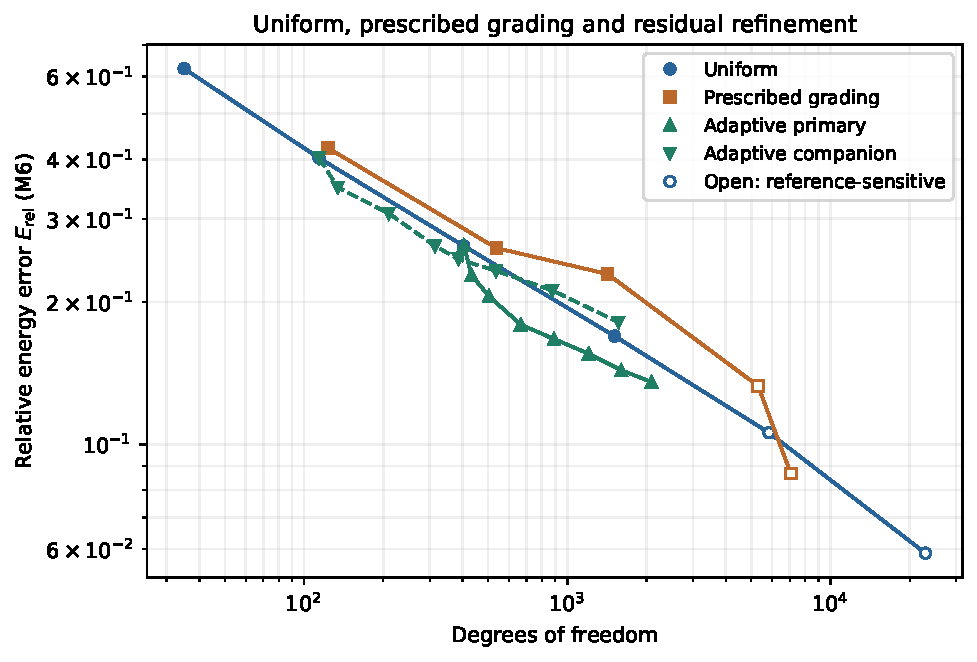
\includegraphics[width=0.92\linewidth]{../figures/adaptive_extension/adaptive_dofs_slide.pdf}
    \end{column}
  \end{columns}
  \begin{alertblock}{Matched-error result: $E_{\rm rel}=0.30$}
    About $18\%$ fewer DOFs than uniform, but $1.83\times$ the cumulative time.\\
    M0-S companion; exact-overlay M6 error with M7 reference check.
  \end{alertblock}
\end{frame}

% ---------------------------------------------------------------------
\section{Final quantities}
% ---------------------------------------------------------------------

\begin{frame}{Final capacitance selection}
  \begin{columns}[T]
    \begin{column}{0.63\textwidth}
      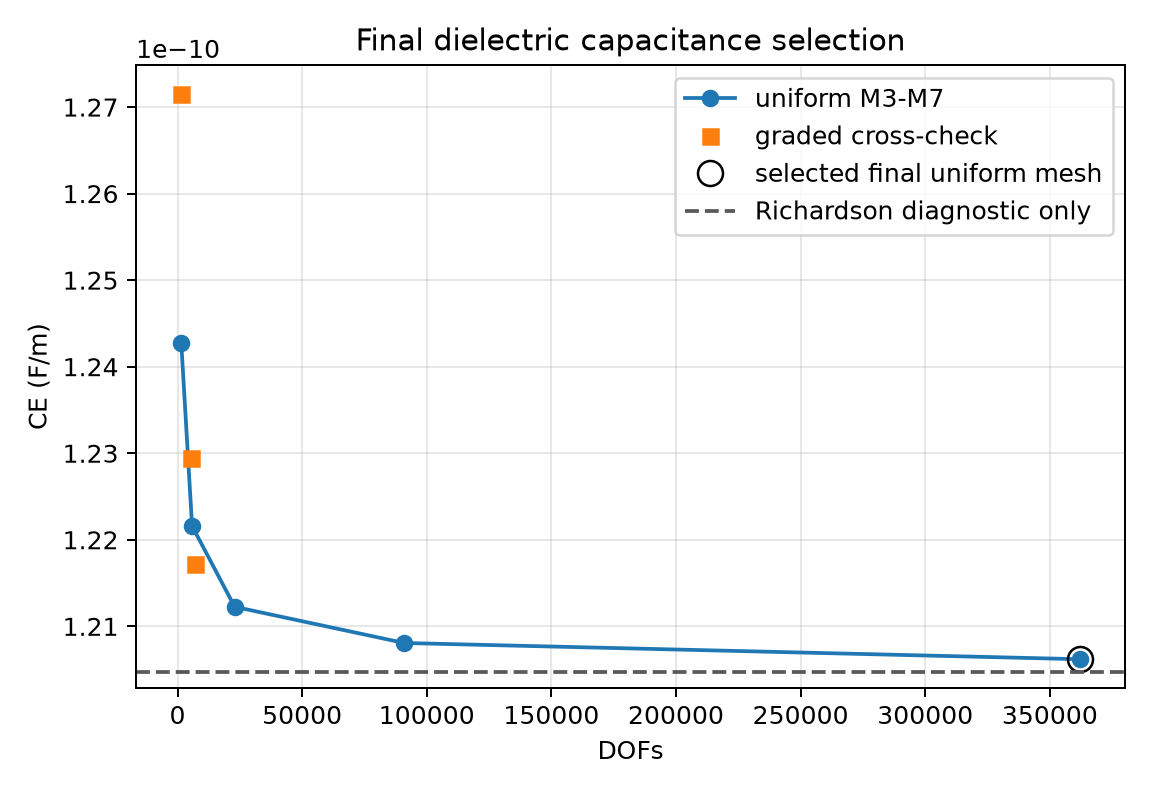
\includegraphics[width=\linewidth]{final_capacitance_convergence.png}
    \end{column}
    \begin{column}{0.33\textwidth}
      \begin{block}{Selected result}
        Uniform M7, 8H domain
        \[
          C=120.620\,\mathrm{pF/m}
        \]
        M6$\to$M7 change: $0.156\%$\\
        Preferred QC target: $0.1\%$
      \end{block}
      \begin{block}{Why M7?}
        \begin{itemize}
          \item Monotone capacitance convergence
          \item Stable asymptotic trend
          \item M8 rejected after resource preflight
          \item Richardson extrapolation is diagnostic only
        \end{itemize}
      \end{block}
    \end{column}
  \end{columns}
\end{frame}

\begin{frame}{Matched all-air solve and effective permittivity}
  \begin{columns}[T]
    \begin{column}{0.57\textwidth}
      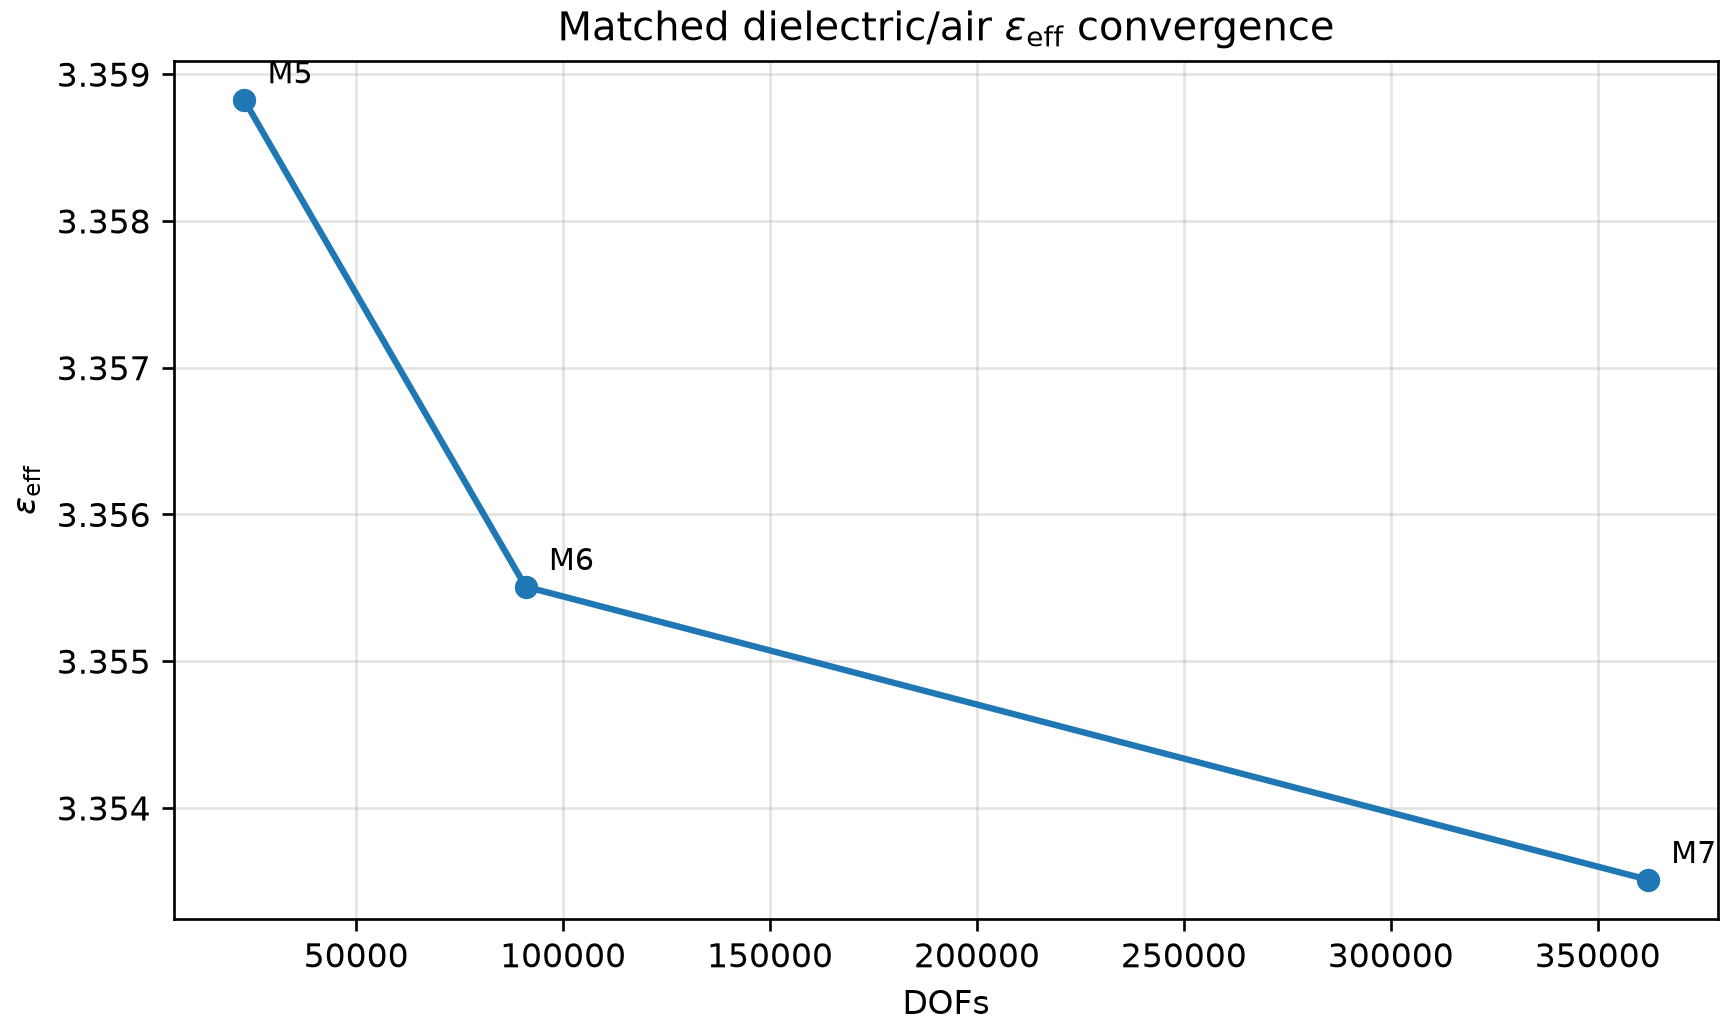
\includegraphics[width=\linewidth]{epsilon_eff_convergence_report.png}
    \end{column}
    \begin{column}{0.39\textwidth}
      \begin{block}{Same frozen mesh}
        The all-air solve reuses the exact M7 mesh from the final dielectric case.
      \end{block}
      \begin{block}{Matched capacitance ratio}
        \[
          \Cair=35.9682\,\mathrm{pF/m}
        \]
        \[
          \epseff=\frac{C}{\Cair}=3.3535
        \]
      \end{block}
    \end{column}
  \end{columns}
  \begin{alertblock}{Takeaway}
    Mesh identity protects the ratio $C/\Cair$ from a hidden remeshing error.
  \end{alertblock}
\end{frame}

\begin{frame}{Final $\Zzero$ and engineering benchmarks}
  \begin{columns}[T]
    \begin{column}{0.56\textwidth}
      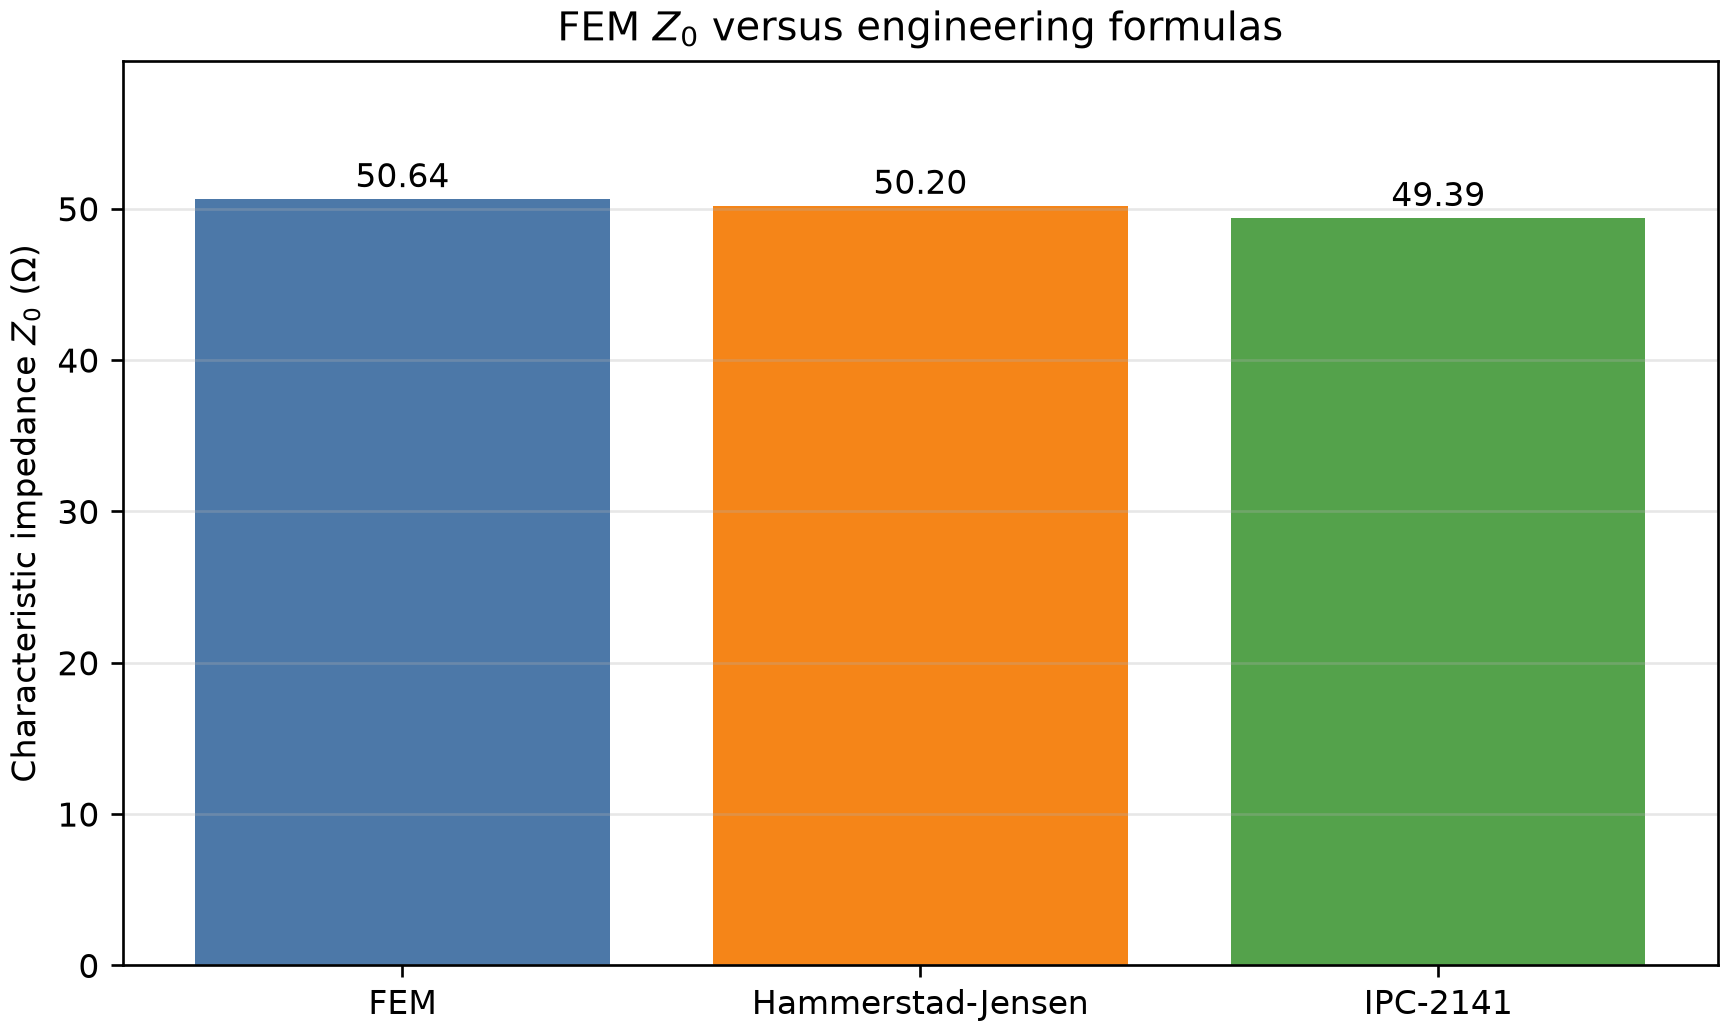
\includegraphics[width=\linewidth]{Z0_benchmark_comparison_report.png}
    \end{column}
    \begin{column}{0.40\textwidth}
      \begin{block}{Quasi-TEM result}
        \[
          \Zzero=\frac{1}{c_0\sqrt{C\Cair}}
          =50.642\,\Omega
        \]
      \end{block}
      \begin{block}{HJ-denominator discrepancy}
        \setlength{\tabcolsep}{3pt}
        \begin{tabular}{@{}lrr@{}}
          \toprule
          Method & $\Zzero$ ($\Omega$) & $100d_{\rm HJ}$\\
          \midrule
          FEM & $50.642$ & $\HJDiscrepancyFEM\%$\\
          HJ (finite $t$) & $50.201$ & $0$\\
          IPC-2141 & $49.393$ & $\HJDiscrepancyIPC\%$\\
          \bottomrule
        \end{tabular}
        \[
          d_{\rm HJ}(Z)=\frac{|Z-Z_{0,\rm HJ}|}{|Z_{0,\rm HJ}|}
        \]
      \end{block}
    \end{column}
  \end{columns}
  \begin{alertblock}{Takeaway}
    Engineering formulas support the scale of the answer, while verification and convergence support the FEM result.
  \end{alertblock}
\end{frame}

% ---------------------------------------------------------------------
\section{Conclusion}
% ---------------------------------------------------------------------

\begin{frame}{Conclusions and limitations}
  \begin{columns}[T]
    \begin{column}{0.48\textwidth}
      \begin{block}{Final reported values}
        \begin{tabular}{@{}lr@{}}
          \toprule
          Quantity & Value\\
          \midrule
          $C$ & $120.620\,\mathrm{pF/m}$\\
          $\Cair$ & $35.9682\,\mathrm{pF/m}$\\
          $\epseff$ & $3.3535$\\
          $\Zzero$ & $50.642\,\Omega$\\
          \bottomrule
        \end{tabular}
      \end{block}
    \end{column}
    \begin{column}{0.48\textwidth}
      \begin{block}{What the model leaves out}
        \begin{itemize}
          \item Losses, surface roughness and fabrication tolerances are omitted.
          \item The quasi-static model does not capture full-wave dispersion or radiation.
          \item Finite-domain and spatial-discretisation sensitivity remain.
        \end{itemize}
      \end{block}
    \end{column}
  \end{columns}
  \vspace{0.6em}
  Residual adaptivity reduced approximation size at $E_{\rm rel}=0.30$, but not cumulative runtime.
  \begin{alertblock}{Main message}
    This is not just a FEM result. It is a verified numerical evidence chain from PDE model to engineering impedance.
  \end{alertblock}
\end{frame}

\end{document}
